\documentclass{MPEtemplate}
% 中文标题
\CNtitle{近代物理实验报告 \LaTeX{} 模板%
 \thanks{本项目没有受到任何资助（这里其实是用来写实验相关信息的）}%
}
% 中文作者
\CNauthor{
  李宇豪\thanks{\email{liyh536@mail2.sysu.edu.cn}}\qquad%
  没有人\thanks{（虚假的）实验合作者}
}
% 中文通讯地址
\CNaddress{中山大学物理学院，广东广州，510275}
% 中文日期
\CNdate{\zhtoday}

% 英文标题
\ENtitle{\LaTeX{} Template of Modern Physics Experiment Report}
% 英文作者
\ENauthor{Yuhao Li and nobody}
% 英文通讯地址
\ENaddress{School of Physics, Sun Yat-sen University, Guangzhou, Guangdong, China}
% 英文日期
\ENdate{\today}

% 中文摘要
\CNabstract{%
这是作者制作的一个用于中山大学近代物理实验报告的LaTeX模板，你可以通过访问 \href{www.http://lyhspace.com/blog/2023/09/06/MPEtemplate/}{lyhspace.com} 下载该模板的项目文件。该模板基于article文档类重新制作了.cls类文件，采用中文单栏排版，制作了独立的标题页放置中英文标题、作者、摘要。该模板样式仅代表作者个人审美喜好，模板内容高度定制化，没有设置封装接口。你可以在遵循 \href{https://creativecommons.org/licenses/by-nc-sa/4.0/deed.zh}{CC BY-NC-SA 4.0} 协议的基础上自由地使用、修改、转发该模板，但是不得用于商业用途或非法转售。如果你有任何问题或者建议，请联系作者。
}
% 中文关键词
\CNkeyword{实验报告，模板，LaTeX}

% 英文摘要
\ENabstract{%
This is a LaTeX template made by the author for the report of modern physics experiments in Sun Yat-sen University. You can download the project file of this template by visiting \href{www.lyhspace.com}{lyhspace.com}. Based on the \textbf{article} document class, the template recreates the \textbf{.cls} file, adopts Chinese single-column typesetting, and makes an independent title page to place Chinese and English titles, authors and abstracts. The template style only represents the author's personal aesthetic preference, and the template content is highly customized, and there is no packaging interface. You are free to use, modify and forward this template on the basis of following the agreement \href{https://creativecommons.org/licenses/by-NC-sa/4.0/deed.zh}{CC BY-NC-SA 4.0}, but it shall not be used for commercial purposes or illegally resold. If you have any questions or suggestions, please contact the author.
}
% 英文关键词
\ENkeyword{Experiment report, Template, LaTeX}

%%%%%%%%%%%%%%%%%%%%%%%%%%%%%%%%%%%%%%%%%%%%%%%%%%
\begin{document}
\maketitlepage
% 正文开始了
%%%%%%%%%%%%%%%%%%%%%%%%%%%%%%%%%%%%%%%%%%%%%%%%%%

\section{一级标题}

正文内容

\subsection{二级标题}

正文内容

\subsubsection{三级标题}

正文内容

\section{示例}

\subsection{插入图片}

这是一张图片。

\begin{figure}[ht]
  \centering
  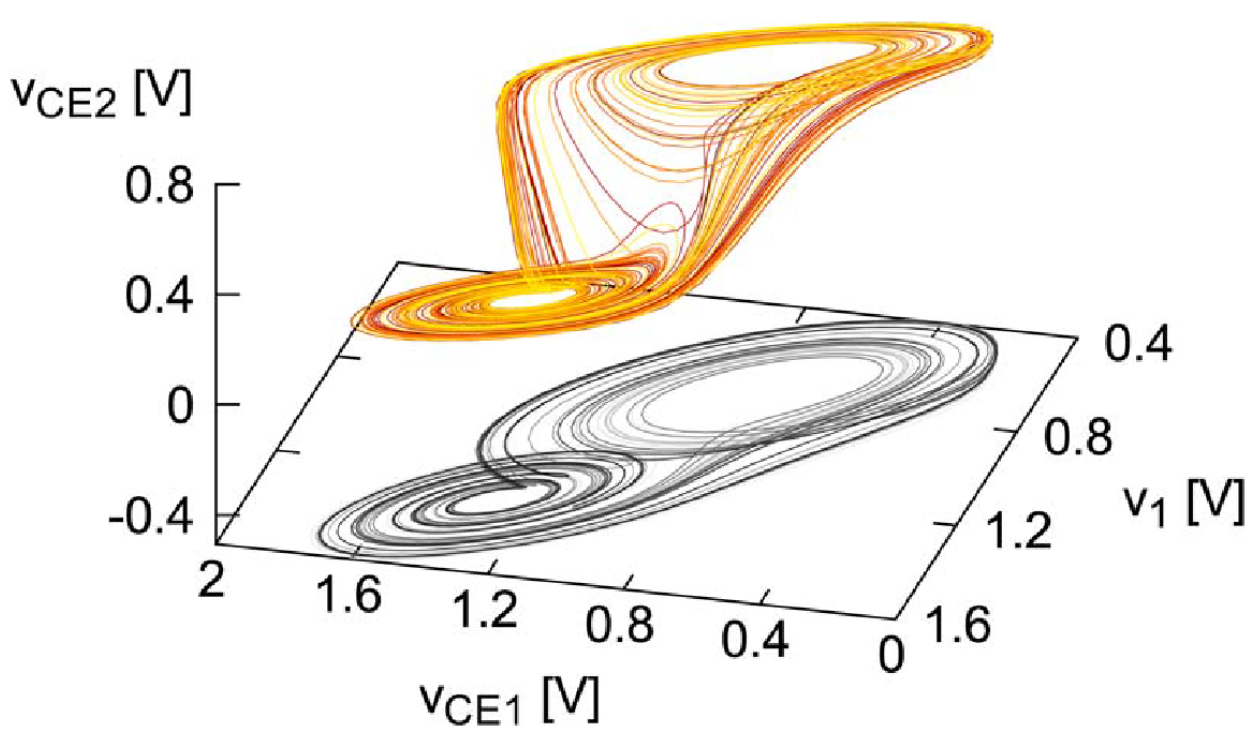
\includegraphics[width=8cm]{img/simp_ref.png}
  \caption{这是一张图片的标题}
\end{figure}

\subsection{插入表格}

这是一个表格。

\begin{table}[H]
\caption{这是一个表格的标题}
\centering
\begin{tabular}{cccc}
\toprule
Item1 & Item2 & Item3 & Item4 \\
\midrule
Data1 &Data2 &Data3 &Data4 \\
Data5 &Data6 &Data7 &Data8 \\
\bottomrule
\end{tabular}
\end{table}

\subsection{数学公式}

这是一个数学公式。

\begin{equation}
    \frac{\mathrm{d} U_{C_1}}{\mathrm{d}  t}=\frac{1}{R_1 C_1} \left(U_{C_2}-U_{C_1}\right)-\frac{1}{C_1} f\left(U_{R_N}\right)
\end{equation}

\subsection{代码}

这是一段python代码

\lstinputlisting[style=python]{pythonCode.py}

这是一段matlab代码

\lstinputlisting[style=matlab]{matlabCode.m}

\subsection{参考文献示例}

这是一句话\cite{edwards1975theory}。

%%%%%%%%%%%%%%%%%%%%%%%%%%%%%%%%%%%%%%
\printbibliography
\beginAppendix
%%%%%%%%%%%%%%%%%%%%%%%%%%%%%%%%%%%%%%
请注意，由于 appendix 宏包与 ctex 宏包冲突，如果你希望附录的一级标题使用 A、B、C… 编号，需要使用 \lstinline|\section*{}| 命令创建一级标题并手动编号，如下所示

\section*{A~~~这里是附录一级标题}

如果你能接受附录的一级标题重新使用 1、2、3… 编号，可以使用 \lstinline|\section{}| 命令创建一级标题，效果如下

\section{这也是附录一级标题}

附录的二级和三级标题同理。

\subsection*{A.1~~~这里是附录二级标题}

附录内容

\end{document}
